\chapter{Implementering}
\label{chap:implementering}

Dette kapitel har til formål at give læseren et indblik i hvilke metoder og teknologier, der er blevet brugt til udviklingen af \Foodl. Teknologierne, som indbefatter bl.a. Ruby on Rails, JavaScript og CSS osv., vil vi ikke gå i dybden med, men blot introducere kort. Derudover vil essentielle algoritmer, samt tankerne bag disse, blive forklaret, og webapplikationen vil blive præsenteret, for at give et overblik over, hvordan {\Foodl} fungerer. 

\section{Teknologier}
\label{sec:teknologier}
Systemet er en webapplikation, hvor der er lagt vægt på enkelt og forståeligt design, effektivitet, fleksibilitet og brugbarhed. For at kunne opfylde alle disse krav og kriterier, som er beskrevet i \secref{sec:kriterier}, har vi gjort brug af nogle forskellige webudviklings- og programmeringsteknologier.

Vi har brugt følgende teknologier:

\begin{itemize}[noitemsep]
\item HTML og CSS
\item Javascript, jQuery UI, AJAX og JSON
\item Ruby on Rails
\item MySQL og phpMyAdmin
\end{itemize}

Vi har brugt HTML\cite{htmlwiki} til at opmærke og strukturere hjemmesiden med. HTML fungerer godt til opmærkning og strukturering af en hjemmeside, men det er ikke særlig flot at se på. For at designe hjemmesiden har vi brugt CSS\cite{csswiki}, der er et sprog, som bruges til at beskrive, hvordan man ønsker indholdet af bl.a. et HTML-dokument skal præsenteres i \fx en webbrowser.

Hvad angår databaser, så har vi har brugt MySQL\cite{mysqlwiki}, der er en flertrådet SQL-databaseserver, som understøtter flere samtidige brugere. I og med at vi består af en gruppe af individer med vidt forskellige kompetencer og erfaringer med web- og systemudvikling, har vi brugt det browserbaserede program, phpMyAdmin\cite{phpmyadminwiki}, til at administrere og opdatere MySQL-databasen. phpMyAdmin præsenterer en letforståelig brugergrænseflade til redigering af databasen. Udviklerne bag MySQL har også udviklet deres eget administrationsmodul til databasen, men den skal installers på en computer, hvorimod phpMyAdmin præsenteres direkte via webbrowseren, hvilket betyder, at vi ikke behøver installere et program på seks forskellige computere, men blot kan bruge det via webbrowseren.

For at gøre hjemmesiden dynamisk og brugervenlig, har vi brugt JavaScript\cite{javascriptwiki}, som er et objektorienteret scriptsprog, som de fleste moderne webbrowsere forstår. Derudover har vi også brugt jQuery UI\cite{jqueryuiwiki}, der bruges til at udvikle interaktive webapplikationer, og AJAX\cite{ajaxwiki} og JSON\cite{jsonwiki}, som bruges til at udvikle asynkrone webapplikationer. Figur \ref{fig:toolbar} illustrerer tre forskellige jQuery UI applikationer, som brugeren bliver præsenteret for, når der bliver udført en søgning på foodl-hjemmesiden. AJAX gør det muligt at udveksle data mellem hjemmeside og server uden at siden skal gennemgå en fuld sideopdatering hver gang, der sker en overførsel, for at vise det nye indhold. Alle dataoverførsler sker i baggrunden og brugeren præsenteres med disse ændringer med det samme.

\begin{figure}[H]
\centering
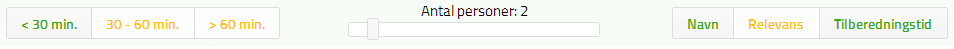
\includegraphics[scale=0.6]{billeder/jqueryuieksempel.png}
\capt{Figuren viser tre forskellige eksempler af interaktive applikationer, der er lavet vha. jQuery UI. Til venstre ses en samling af tre knapper, som fungerer som afkrydsningsbokse, hvilket betyder, at man kan markere flere af gangen. Disse knapper gør det muligt for brugeren at begrænse søgeresultatet efter disse tre kriterier for tilberedningstiden. Midt for ses en justerbar knap, der gør det muligt for brugeren at skalere opskrifterne. Til højre ses endnu en samling af tre knapper, der fungerer som radioknapper, hvilket betyder, at man kun kan vælge én knap af gangen. Disse knapper giver brugeren mulighed for at sortere resultaterne efter navn, relevans eller tilberedningstid.}
\label{fig:toolbar}
\end{figure}

Derudover har vi anvendt Ruby on Rails \cite{rubyonrailswiki}, der er et webudviklingsframework baseret på programmeringssproget Ruby, til at understøtte webudviklingen. Intentionerne bag Rails var at skabe et framework, der gjorde det lettere og hurtigere for webudviklere at udvikle webapplikationer, hvilket også er en af de væsentlige årsager til, at vi valgte at anvende Rails. 

Målet med Rails blev bl.a. opnået vha. af følgende filosofi:
\begin{quote}
``konventioner over konfigurationer''
\end{quote} 

Filosofien har både sine fordele og ulemper. Det er en ulempe, at webudvikleren skal have arbejdet meget med Rails i forvejen, for at kunne huske de mange konventionerne og kommandoer, eller bruge en masse tid, på at slå dem op, når de skal bruges. Det er på den anden siden en fordel, at webudviklere, vha. Rails' konventioner, kan lave applikationer, som kan udrette meget, ud fra få linjers kode. Rails viser allerede fra første møde, at der skal meget lidt arbejde til, for at få et stort afkast. Dette kan ses på \figref{fig:Rails-new-foodl}, hvor en enkelt linje i kommandoprompten, genererer en ny mappe, som indeholder en funktionsdygtig Railsapplikation, kaldet ``Foodl''.

\begin{figure}
	\centering
	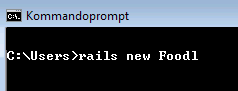
\includegraphics[scale=0.6]{billeder/Rails-new-foodl.png}
	\capt{Railskommando, der indtastes i kommandopromten, hvorefter rails genererer en mappe med en fuldtfungerende web-applikation, kaldet ``Foodl''}
	\label{fig:Rails-new-foodl}
\end{figure}

Enhver Railsapplikation tager udgangspunkt i arkitekturen Model-View-Controller. Mappen med webapplikationen består af en lang række undermapper, hvori ``models'', ``views'' og ``controllers'' bl.a. befinder sig. Kort sagt genererer Rails, vha. \texttt{new}-kommandoen, hele skelettet for webapplikationen, og derefter er det ``bare'' at fylde det indhold, man ønsker i sin webapplikation, i de rigtige mapper. Denne Model-View-Controllerarkitektur vil blive forklaret yderligere i følgende \secref{subsec:mvc}.

\subsection{Model-View-Controller}
\label{subsec:mvc}
3-lag arkitekturen minder meget om Model-View-Controller mønstret, som vi benytter og har kort beskrevet i \secref{subsec:mvc}. Dog skal det nævnes, at de ikke er helt ens. I en 3-lags komponentarkitektur er det ikke muligt for præsentationslaget at tilgå modellen. MVC-mønstøret er mere trekantet idet, at views kan tilgå både funktionskomponenten og modelkomponenten og dermed blive opdateret direkte fra modellen\cite{designpatterns}. MVC-arkitekturen kan ses i \figref{fig:komponenter}. Der findes mange forskellige frameworks, der bygger på MVC-arkitekturen. Fordelen er ved at benytte et eksisterende og anerkendt framework, er dets mange funktioner og brugervenlighed, der gør det muligt at hurtigt kunne implementere de nødvendige dele af systemet.

Arkitekturen består af tre hovedkomponenter: model, view og controller. Modelkomponenten bærer de data, som typisk er repræsenteret som tabeller i en database, der skal kunne manipuleres. Controllerkomponenten fungerer som et slags bindeled mellem modellen og views ved at sende forespørgsler til modellen eller views, alt afhængig af brugerinputtet fra de tilsluttede views. Derudover sender controlleren også forespørgsler i form af tilstandsændringer til modellen, hvis brugeren \fx opdaterer noget i et view. Et view præsenterer brugeren for data i modellen og muliggør ændringer i tilstanden af modellen.

Vi benytter også klient-server arkitekturmønstret, se \figref{railsmvc} der er oplagt, netop fordi vores model består af rigtig mange opskrifter. Det vil være upraktisk at overføre alle opskrifterne til hver eneste bruger, der benytter systemet, da det vil give en stor belastning på systemet og stor ventetid for brugeren. Vi lader derfor webbrowserkomponenten fungere som klient og tilkobler sig serveren under for at sende forespørgsler. Det er controller-komponenten, der sørger for at sende data frem og tilbage mellem klienten og server. Der er altså kun én server, som integrerer med mange forskellige klienter igennem et netværk og deler fælles ressourcer med alle de klienter, der er tilkoblet. Serverkomponenten stiller diverse funktioner tilgængelig for klienterne, \fx at muliggøre søgning eller lagring af oplysninger i modelkomponenten. Serveren, i dette tilfælde, og i modsætning til klient-servermønstret beskrevet i OOA\&D\cite{ooad}, kan godt kende noget til/om klienten. \Fx er det muligt, at vise andre views, alt afhængigt af hvilken webbrowser, der bliver tilkoblet serverkomponenten.

\pdffig[0.7]{railsMVC}{Et tilpasset generiske Model-View-Controller mønster indkapslet i et klient-server arkitekturmønster\cite{railsmvc}.}{fig:railsmvc}


\section{Funktionalitet}
\label{sec:funktionalitet}

Da {\Foodl} er en Railsapplikation består den, som andre MVC-applikationer, hovedsageligt af modeller, controllers og views. Modeller er klasser, der repræsenerer data, dvs. f.eks. tabeller i databasen. Controllers er klasser bestående af actions, eller handlinger, som er metoder, der har til formål at reagere på en aktørs interaktion med serveren. Den sidste grundlæggende del af MVC-designet er views, som er template-filer, som bliver udfyldt med data gennem controlleren og sendt tilbage til aktøren. I {\Foodl} er der flest HTML-templates, som har til formål at præentere data i brugerens webbrowser.

Derudover blabla helpers.. assets.. osv\todo{}

\subsection{Controllers}
\label{sec:controllers}

{\Foodl} består af følgende controllers:

\begin{description}
  \item[ApplicationController] \hfill \\ 
  Den overordnede applikationscontroller, som alle andre controllers i Foodl nedarver fra. Den kan f.eks. indeholde forskellige helper-metoder, som skal kunne tilgås overalt i applikationen.

  \item[FavoritesController] \hfill \\ 
  Denne controller håndterer brugerens favoritter, hvad enten denne er logget ind eller ej. Controlleren har tre actions, en til at liste favoritter, en til at tilføje favoritter og en til at fjerne favoritter.

  \item[HomeController] \hfill \\ 
  Denne controller håndterer applikationens to statiske sider, "Om foodl" og "Kontakt foodl".

  \item[IssuesController] \hfill \\ 
  Fejlhåndteringen foregår med denne controller. Dvs. oprettelsen af fejlrapporter og listen af disse.

  \item[RecipesController] \hfill \\
  Kun én action er indeholdt i denne controller, en action til at servere det billede der hører til en opskrift.

  \item[SearchController] \hfill \\
  Søgning håndteres i denne controller. Søgningen er beskrevet i detaljer i \secref{sec:funktionalitet-soegning}.

  \item[SessionsController] \hfill \\
  Denne controller håndtere brugersessioner, dvs. når en bruger vil logge ind eller ud.

  \item[ShoppingListController] \hfill \\
  Indkøbslisten håndteres med denne controller. Tilføjelsen af elementer, hvad enten det er ingredienser, rå tekststrenge eller hele opskrifter, samt sletning af elementer muliggøres af denne controller.

  \item[UsersController] \hfill \\
  Denne controller håndtere alt i forbindelse med brugere, dvs. f.eks. opretning af bruger, opdatering af kodeord og funktionen "Glemt kodeord".

\end{description}

\subsection{Modeller}

\begin{description}

  \item[FoodType] \hfill \\
  Råvare

  \item[Ingredient] \hfill \\
  Ingrediens

  \item[IssueCategory] \hfill \\
  Fejltype

  \item[Issue] \hfill \\
  Fejlrapport

  \item[ListItem] \hfill \\
  Vare

  \item[Recipe] \hfill \\
  Opskrift

  \item[User] \hfill \\
  Bruger

\end{description}
\todo{WIP}
\subsection{Tabeller}
\label{sec:tabeller}

Hver model svarer til en tabel i databasen. Vores tabelstruktur kan ses i \figref{fig:database}. \dbtableref{sessions}-tabellen bruges af en intern Session-model i Rails, som er nødvendig for at gemme sessionsdata på serveren.

Ydermere er der tabellen \dbtableref{users\_recipes}, som er nødvendig for at udtrykke mange-til-mange-forholdet mellem brugere og opskrifter. Dvs. at hver relation mellem en bruger og en opskrift (en favorisering) svarer til en række i denne tabel, som indeholder både et id for en opskrift og et id for en bruger. Når tabellen først er oprettet sørger Rails selv for at abstrahere denne relation, sålænge en \methodref{has\_and\_belongs\_to\_many}-relation, der peger på User-modellen, er sat op i Opskrift-modellen og vice versa. Dette medvirker at man f.eks. nemt kan tilføje en opskrift til en brugers favoritter vha. en enkelt linje Ruby-kode, som illustreret i \lstref{list:rubymanytomany}.

\begin{lstlisting}[caption={Hvis man har et \classref{User}-objekt i \texttt{user} (som f.eks. returneret med \lstinline{User.find_by_id(42)}) og et \classref{Recipe}-object i \texttt{recipe}, kan opskriften associeres med brugeren med denne linje Ruby-kode.},label=lst:rubymanytomany,language=Ruby]
user.favorites << recipe
\end{lstlisting}
\todo{WIP}
\pdffig{database}
  {Databasetabelstrukturen og associeringerne mellem tabellerne.}
  {fig:database}

\subsection{Søgning}
\label{sec:funktionalitet-soegning}
Søgningen må siges at være den vigtigste del af \Foodl. Som beskrevet i \classref{sec:systemdefinition}, så er målet med projektet netop at kunne søge blandt mange opskrifter og returnere de opskrifter, som indeholder de råvarer, som brugeren har valgt.

Alt dette styres af klassen \classref{SearchController}, som består af tre actions. Ligeledes er aktiviteten spredt ud over to views; \methodref{index}, som er er selve forsiden af \Foodl med mulighed for at indtaste ingredienser, og \methodref{result}, som er resultatsiden.

Den tredje action i controlleren er \methodref{autocomplete\_food\_types}, hvortil der ikke er tilknyttet et view. Denne action har til formål at returnere en liste over råvarer baseret på brugerens indtastning. Denne funktionalitet er beskrevet i detaljer i nedenstående afsnit.

\subsubsection{Søgeforslag}
En central del af forsiden, og brugerens mulighed for at vælge råvarer, er at systemet kommer med en liste over forslag, baseret på brugerens indtastning. \todo{WIP}

\begin{lstlisting}[caption={SQL query.},label=lst:soegeforslag-sql,language=SQL]
SELECT name
FROM food_types
WHERE name LIKE "%pølse%"
ORDER BY CASE
    WHEN name LIKE "pølse" THEN 1
    ELSE 0
  END DESC,
  CASE
    WHEN name LIKE "pølse%" THEN 1
    ELSE 0
  END DESC,
  LENGTH(name) ASC
LIMIT 5
\end{lstlisting}

Resultatet af SQL-forespørgslen i \lstref{lst:soegeforslag-sql} er en liste med 5 forslag til råvarer. Listen sorteres således at hvis der findes et forslag, der matcher det indtastede 100 \%, vil dette komme øverst (den første \texttt{CASE} i \lstref{lst:soegeforslag-sql}). Dernæst rangeres forslag, som starter med det indtastede, højere end forslag, som ikke starter med det indtastede.

\subsubsection{Søgeresultat}
\todo{WIP}
\begin{lstlisting}[caption={SQL query.},label=lst:soegeforslag-sql,language=SQL]
SELECT recipes.*, COUNT(*) AS relevance
FROM ingredients
RIGHT JOIN recipes ON recipe_id = recipes.id
WHERE food_type_id IN ( 2, 23, 12 )
GROUP BY recipes.id
ORDER BY relevance DESC
LIMIT 0, 50
\end{lstlisting}


\section{Brugergrænseflade}
\label{sec:webapplikationen}
Vi har udviklet en webapplikation, som vi har valgt at kalde \Foodl. I dette afsnit bliver webapplikationen præsenteret og beskrevet.

Vi har valgt at gøre designet så enkelt som muligt for ikke at forvirre brugerne. Når man kommer taster sig ind på hjemmesiden \url{http://www.foodl.dk}, bliver man mødt af en velkomsthilsen, der meget kort beskriver hjemmesidens formål og brug. Denne hilsen kan bruge vælge at lukke ned. En cookie bliver gemt i browseren, så velkomsthilsnen ikke bliver vist igen, medmindre browserhistorikken bliver ryddet.

Figur \ref{fig:foodl-forside} viser forsiden af hjemmesiden, uden velkomsthilsnen. Navnet \Foodl er også en del af webapplikationens logo. For at gøre det mere klar for en ny bruger, hvad siden handler om, så har vi erstattet et O i navnet med en stor ananas, fordi det er noget, der kan spises, og sidens formål er at give folk mulighed for at genbruge deres madrester. 

\begin{figure}[H]
	\centering
	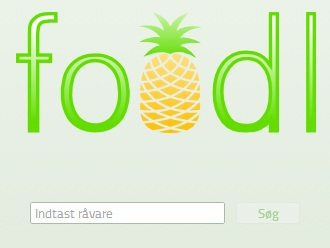
\includegraphics[scale=0.7]{billeder/foodl/forside.jpg}
	\capt{Denne figur viser webapplikationens startside. Logoet med den store ananas, der skal forestille bogstavet O, har til formål at byde brugerne velkomne til siden. Direkte under logoet kan brugerne indtaste de råvarer, de ønsker at bruge til madlavningen.}
	\label{fig:foodl-forside}
\end{figure}

På alle undersider af \url{foodl.dk} er det muligt at tilgå sidehovedet. Her er der mulighed for at navigere tilbage til forsiden ved at klikke på den mindre version af det store logo, som blev vist på forsiden. Derudover kan man tilgå både en indkøbsliste og en liste af favorit-opskrifter, som brugeren selv vælger fra hjemmesiden. Både indkøbslisten og favoritter har et tal i parentes, der \fx fortæller brugeren, hvor mange varer, der er i den nuværende indkøbsliste eller hvor mange opskrifter, der er gemt under favoritter. Dette kan ses på \figref{fig:foodl-header}.

Ydermere kan man se på \figref{fig:foodl-header}, at det er muligt at logge ind eller oprette en bruger i webapplikationen. Dette er dog ikke obligatorisk, da vi ikke ønsker at binde brugerne til at oprette noget som helst. Man kan bruge systemet, om man har en bruger eller ej. Den eneste fordel ved at oprette en bruger er, at man på denne måde kan gemme indkøbslisten og favoritterne under hver bruger til fremtidigt brug.

\begin{figure}[H]
	\centering
	
\includegraphics[scale=0.7]{billeder/foodl/header.jpg}
	\capt{Denne figur viser webapplikationens sidehoved, hvilket kan ses på alle undersider. Herfra kan forsiden (foodl), indkøbslisten og favoritter tilgås. Derudover er der mulighed for at brugeren kan logge ind eller oprette en bruger. Dette er frivilligt. Systemet kan godt bruges uden at oprette en bruger.}
	\label{fig:foodl-header}
\end{figure}

Som sagt så har brugeren ikke behov for at logge ind for at bruge systemet. Det er nu op til brugeren at indtaste alle de råvarer, der ønskes brugt til madlavningen. Figur \ref{fig:foodl-soegefelt} viser, hvordan en sådan søgning foregår. Der bliver løbende indtastet bogstaver, og systemet undersøger for dele af tekststrenge, der matcher det der bliver indtastet. Ud fra disse match gives der forslag til hvilke råvarer, man kan vælge. Man kan ikke indtaste hvad som helst som et søgekriterie i systemet. Der er en lang række råvarer at vælge imellem. Hvis der \fx bliver indtastet kød i søgefeltet, så kommer der en liste af matchende råvarer som forslag, som man kan se på \figref{fig:foodl-soegefelt}.

For at fuldføre en søgning skal man blot trykke på ``Søg'', der er til højre for søgefeltet. Når brugeren trykker ``Søg'', så arbejder systemet på at finde alle de opskrifter, der minimum har en ingrediens, der matcher en af de indtastede råvarer.

\begin{figure}[H]
	\centering
	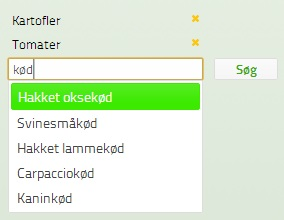
\includegraphics[scale=0.7]{billeder/foodl/soegefelt.jpg}
	\capt{Denne figur viser webapplikationens søgefelt. Når brugeren begynder at stave til de råvarer, der ønskes at blive brugt i madlavningen, så giver webapplikationen forslag til råvarer, der er søgbare i systemet, som indeholder lignende tekst-dele, hvilket brugeren løbende bliver indtaster i feltet. Der er også mulighed for at slette valgte råvarer ved at trykke på de små gule krydser ud for råvaren. Når brugeren har valgt alle de råvarer, der ønskes brugt, så skal brugeren trykke på Søg-knappen for at fuldføre søgningen.}
	\label{fig:foodl-soegefelt}
\end{figure}

Det er efter denne søgning, at brugeren finder ud af, hvad der er muligt at lave ud fra de råvarer, der er til rådighed. Resultatet er selvfølgelig afgrænset til den database man har over opskrifter.

Når søgningsresultatet vises, så er det en liste af opskrifter. I første omgang er opskrifterne sorteret efter relevans, dvs. hvor mange ingredienser, der matcher de forskellige indtastede råvarer. Figur \ref{fig:foodl-opskrift} viser et eksempel af en opskrift, der er et resultat af den foretagede søgning. I eksemplet er der kun 1 ingrediens, der matcher de indtastede råvarer, og denne er markeret med fed skrift (semidried tomatoes).

På hjemmesiden vises der kun hvilke ingredienser, der skal til for at lave opskriften, men selve fremgangsmåden er ikke vist nogen steder. Man er nødt til at tilgå den oprindelige hjemmeside, hvorfra opskriften stammer fra. Dette gøres ved at trykke på enten opskriftens titel eller billedet. Begge elementer består af et link til opskriftens originale hjemmeside. 

Fremgangsmåden kan ikke ses på vores hjemmeside, men alle andre vigtige elementer af opskriften er synlige. En opskrift består af følgende elementer:

\begin{itemize}[noitemsep]
\item Titel
\item Billede
\item Tilberedningstid
\item Relevans (antal matchende ingredienser)
\item Ingredienser
\item Knapper
\begin{itemize}[noitemsep]
\item Tilføj alle ingredienser til indkøbsliste
\item Tilføj / fjern fra favoritter
\item Tilføj enkelte ingredienser til indkøbsliste
\item Indmeld en fejl med opskriften
\end{itemize}
\end{itemize}

Alle opskrifter består af en beskrivende titel og et relevant billede, der skal vise brugeren, hvordan opskriften kan se. Billedet er med til at vække en interesse hos brugeren. Tilberedningstiden er også en vigtig ting at være klar over, og denne kommer direkte under billedet. De matchende ingredienser er markeret med fed skrift, så har brugeren nemmere ved at gennemskue, hvad der \fx er relevant at handle ind ud fra alle ingredienserne. Derudover er der et sæt knapper, som brugeren kan bruge. Se \figref{fig:foodl-opskrift}. I øverste højre hjørne er der en knap, der har et notesblok-lignende ikon. Denne knap tilføjer alle ingredienserne til indkøbslisten. Der er også mulighed for at tilføje de enkelte ingredienser ved at trykke på de små plus'er ud for ingredienserne. Ydermere er der mulighed for at tilføje og fjerne en opskrift til ens favorit-liste. Dette gøres ved at trykke på den hjerte-formede knap. I nederste højre hjørne er der en advarselsknap, der bruges til at rapportere om eventuelle fejl ved den specifikke opskrift.

\begin{figure}[H]
	\centering
	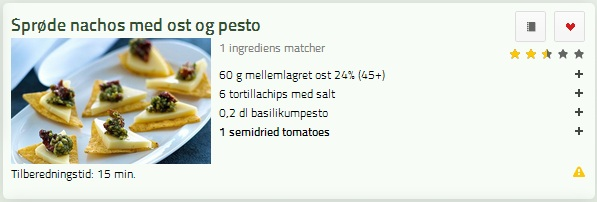
\includegraphics[scale=0.7]{billeder/foodl/opskrift.jpg}
	\capt{Når brugeren fuldfører en søgning, så bliver brugeren præsenteret med en liste af opskrifter, der minimum indeholder en ingrediens, der passer med en af de råvarer, som blev indtastet af brugeren. Her ses en opskrift ud af en liste af opskrifter, som var resultatet af søgningen, der blev foretaget. Et søgeresultat består af opskriftens titel og billede, hvilket begge er link, der fører brugeren videre til opskriftens fremgangsmåde på dens originale hjemmeside. Direkte under billedet kan man se, hvor lang tid det ca. tager at tilberede opskriften. Derudover kan man se, hvor mange ingredienser, der matcher fra søgningen, og de ingredienser, der matcher er markeret med fed skrift i resultatet. I øverste højre hjørne af resultatet, kan man (ved den hjerteformede knap) tilføje og fjerne en opskrift fra favoritter. Knappen til venstre for hjertet, der er formet som en lille notesblok, tilføjer alle ingredienserne til brugerens indkøbsliste. Direkte under disse to knapper kan man se,hvor mange stjerner en opskrift har fået. Opskrifterne får stjerne ud fra det antal brugere, der har favoriseret opskriften. De små plusser bruges til at tilføje enkelte ingredienser til indkøbslisten. I nederste højre hjørne er der en advarselsknap, som bruges til rapportering af eventuelle fejl med den specifikke opskrift.}
	\label{fig:foodl-opskrift}
\end{figure}

Brugeren har forskellige muligheder for at manipulere søgningsresultatet. Der er blevet implementeret en toolbar i toppen af siden, der følger brugerens bevægelser mht. at scrolle op og ned. På denne måde behøver brugeren ikke at scrolle helt til toppen for at udføre en handling på søgningsresultatet. 

Figur \ref{fig:foodl-toolbar} illustrerer, hvordan toolbaren ser ud. I venstre side er der en samling af tre knapper, der bruges til at begrænse søgningsresultatet mht. tilberedningstiden. Her er der mulighed for at markere flere af gangen, og default kriteriet er, hvis ingen er markeret, så er alle markeret. Dette betyder, at systemet starter med at vise alle resultater. I midten af toolbaren er der et skaleringsværktøj, der kan bruges til at skalere opskrifternes portioner mht. antal personer. Man kan skalere dem ned til 1 person og op til 10 personer. Vi valgte 10 som maximum, fordi det er relativt let at skalere yderligere, hvis dette er ønsket. Til højre er der endnu en samling af tre knapper, men disse benyttes til at sortere opskrifterne. Default er relevans. De to knappesamlinger er forskellige på to måder; hvad de bruges til, og at der kun er mulighed for at markere en knap af gangen ved sorteringsknapperne (højre side) og mulighed for markering af flere af gangen ved afgrænsningsknapperne (venstre side).

\begin{figure}[H]
	\centering
	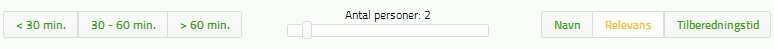
\includegraphics[scale=0.7]{billeder/foodl/toolbar.jpg}
	\capt{Toolbaren er direkte under sidehovedet. I venstre side af toolbaren er der en samling af tre knapper, der kan specificere en søgning ud fra tilberedningstiden. I midten af toolbaren kan man skalere opskrifterne fra 1 til 10 personer. Til højre kan man sortere listen af opskrifter efter navn, relevans eller tilberedningstid. Toolbaren følger vinduet, når man scroller op og ned, så brugeren altid kan manipulere listen af opskrifter efter behov.}
	\label{fig:foodl-toolbar}
\end{figure}

Ud over toolbaren, så viser \figref{fig:foodl-sidebar} en sidebar, hvilket gør det mulight for brugeren at følge med i, hvad der bliver søgt på, og den er en mulighed for brugeren at lave endnu en søgning. Man kan herfra slette og/eller tilføje nye råvarer til en ny søgnign. Denne sidebar følger også brugeres scrolling, da det skal være nemt og hurtigt at lave en ny søgning, hvis dette bliver aktuelt.

\begin{figure}[H]
	\centering
	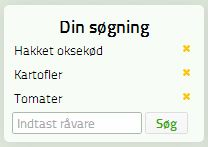
\includegraphics[scale=0.7]{billeder/foodl/sidebar.jpg}
	\capt{Sidebaren er placeret venstre for listen af opskrifter, og bruges til at holde brugeren opdateret med, hvilke råvarer, der er blevet søgt på. Man kan direkte fra denne redigere søgningen og udføre en ny søgning. Sidebaren følger vinduet, når man scroller op og ned, så brugeren altid er klar til at søge igen.}
	\label{fig:foodl-sidebar}
\end{figure}

Hvis en bruger vælger at benytte sig af indkøbslisten, så kan denne tilgås via sidehovedet, som kan ses på \figref{fig:foodl-header}, ved at trykke på ``indkøbsliste''. I sidehovedet kan man også se, hvor mange varer, der er blevet tilføjet til listen. 

Man kan tilføje hvilken som helst tekststreng til indkøbslisten. På denne måde har vi ikke begrænset brugeren til blot at tilføje ingredienser fra opskrifterne, men det er helt op til brugeren selv at bestemme, hvad skal på listen. Brugeren har mulighed for at tilføje varer i feltet ``tilføj til indkøbsliste'' og trykke på ``tilføj''. Der er mulighed for at slette alle varer fra indkøbslisten og ligeledes at slette enkelte varer. Derudover er der implementeret en knap, til at udskrive indkøbslisten, hvis det skulle være nødvendigt.

\begin{figure}[H]
	\centering
	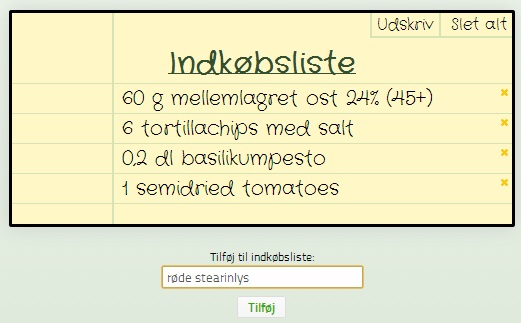
\includegraphics[scale=0.7]{billeder/foodl/indkoebsliste.jpg}
	\capt{Indkøbslisten tilgås fra sidehovedet. Her får brugeren mulighed for at se, hvad der er blevet tilføjet til indkøbslisten og eventuelt tilføje flere varer. I dette eksempel ønskes der at tilføjes røde stearinlys til listen. Brugeren har mulighed for at slette alle varer på listen ved at trykke på knappen i øverste højre hjørne, eller brugeren kan slette enkelte varer, der ikke skal købes. Derudover er der mulighed for at udskrive listen ved at klikke på knappen i øverste højre hjørne.}
	\label{fig:foodl-indkoebsliste}
\end{figure}

I \figref{fig:foodl-opskrift} vises en knap, der bruges til at rapportere eventuelle fejl ved de specifikke opskrifter. Figur \ref{fig:foodl-fejlrapportering} viser, hvordan det ser ud, når en bruger trykker på rapporteringsknappen ved en opskrift. Der popper en lille boks op, og baggrunden af siden bliver mørk. Her kan man nu specificere, hvad fejlen handler om og give en beskrivelse, inden man vælger at indsende fejlen.

\begin{figure}[H]
	\centering
	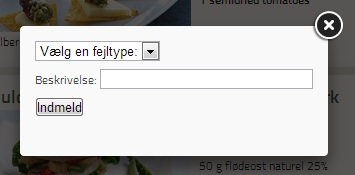
\includegraphics[scale=0.7]{billeder/foodl/fejlrapportering.jpg}
	\capt{Når en bruger opdager en fejl ved en opskrift, så har brugeren muligheden for at indberette fejlen ved at trykke på advarselsknappen, der kan ses i \figref{fig:foodl-opskrift}. Brugeren kan nu vælge en fejltype og beskrive dennne, inden fejlen bliver indmeldt.}
	\label{fig:foodl-fejlrapportering}
\end{figure}

Muligheden for oprettelse af bruger er tilstede. Figur \ref{fig:foodl-opret} viser, hvordan denne ``log ind / opret bruger'' side ser ud. Man skal bruge sin email og en adgangskode for at lave en bruger. Hvis man allerede har en bruger, så skal man blot logge ind med de rigtige oplysninger. Som det tidligere blev nævnt, så er det ikke obligatorisk at oprette en bruger. Den eneste fordel der er ved dette er, at man får mulighed for at gemme indkøbslisten og listen over favoritter. 

Når man er logget ind, så ændrer sidehovedet sig en smule. Figur \ref{fig:foodl-header-loggetind} viser, at der nu er mulighed for at gå ind i en menu, der hedder ``indstillinger'' og at logge ud igen. Man kan også se, at der pludselig er indlæst en liste af favoritter på 10 opskrifter fra tidligere besøg.

\begin{figure}[H]
	\centering
	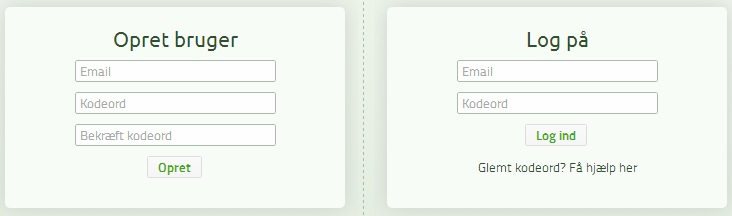
\includegraphics[scale=0.7]{billeder/foodl/login-opret.jpg}
	\capt{Hvis brugeren ønsker der, så kan man oprette en bruger i webapplikationen. Dette gør det muligt at gemme favoriseringer og indkøbsliten til brug i fremtiden eller på andre enheder. Når man trykker på ``log ind / opret bruger'', som kan ses i \figref{fig:foodl-header}, bliver brugeren præsenteret med to valg. Muligheden for at logge ind eller oprette en bruger. Her skal der indtastes e-mail og adgangskode.}
	\label{fig:foodl-opret}
\end{figure}

\begin{figure}[H]
	\centering
	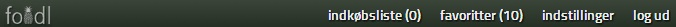
\includegraphics[scale=0.7]{billeder/foodl/header-login.jpg}
	\capt{Når brugeren er logget ind, så ændrer sidehovedet sig en smule. ``log ind / opret bruger'' bliver erstattet med ``indstillinger'' og ``log ud''. Derudover indlæses eventuelle gemte favoritter og indkøbsliste.}
	\label{fig:foodl-loggetind}
\end{figure}

Hvis man ønsker at skifte sin adgangskode, så sker det ved at trykke på knappen ``indstillinger'' i sidehovedet. Dette illustrerer \figref{fig:foodl-indstillinger}.

\begin{figure}[H]
	\centering
	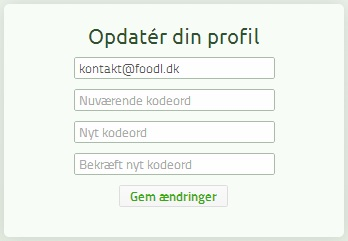
\includegraphics[scale=0.7]{billeder/foodl/indstillinger.jpg}
	\capt{Brugeren har mulighed for at ændre nogle basale indstillinger ved at klikke på ``indstillinger'' i sidehovedet, som kan ses i \figref{fig:foodl-loggetind}. Her kan brugeren ændre sin adgangskode.}
	\label{fig:foodl-indstillinger}
\end{figure}

Som de fleste andre hjemmesider, så har vi også en ``om'' og en ``kontakt'' side, som kan tilgås fra nederste venstre hjørne af enhver foodl-underside. Derudover kan man rapportere en generel fejl ved siden, hvis man støder på sådan en.

\begin{figure}[H]
	\centering
	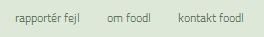
\includegraphics[scale=0.7]{billeder/foodl/formaliteter.jpg}
	\capt{I nederste venstre hjørne af webapplikationen kan man rapportere en generel fejl, læse mere om webapplikationen og kontakte udviklerne.}
	\label{fig:foodl-formaliteter}
\end{figure}

\subsection{Parsing af Opskrifter}
Opskrifterne på Arla blev parset ved brug af modulet Nokogiri i Ruby. Nokogiri-modulet gør det let at finde værdier af forskellige elementer i et dokument. På Arlas hjemmeside findes en side, der giver mulighed for at vise alle opskrifterne. Der vises 16 opskrifter af gangen, og når man bladrer frem og tilbage imellem side 1 og side 2, hver især med 16 forskellige opskrifter på hver, så ændres en query i url'en på følgende måde: \\
\lstinline{?...\&paging=1\&...} \\
\lstinline{?...\&paging=1\&...} \\
En variabel ved navn \textit{paging} ændres i queryen værdi fra 1 til 2. Siderne, der indekserer 16 opskrifter af gangen er derfor lette at finde ved blot at lade en variable gå fra 1 og øges indtil ingen opskrifter fremkommer.

På hver enkelt indekseringsside vises 16 opskrifter. Et link til en opskrift på Arlas indekseringsside, ser i HTML således ud:

\lstinline{<h2><a href="/opskrifter/Suppe">Suppe</a></h2>}

Ved at bruge klassen \textit{xpath} i Nokogiri, kan alle 16 links hurtigt returneres som at array ved at benytte funktionen:

\texttt{xpath("//h2//a").map{|link| "http://www.arla.dk"+link["href"]}}

Metoden \textit{xpath}, leder efter alle \textit{<a>} tags inde i \textit{<h2>} tags og returnerer et array af elementer, der hver især har en værdi for indekset \textit{href}, der svarer til linket til siden. Ved at bruge funktionen \textit{map}, fås værdien af indekset \textit{href}, og præfixet \texttt{http://www.arla.dk} tilføjes foran. En forudsætning, der var til stede, for at kunne benytte denne metode, var at samme tagsekvens, i dette tilfælde \lstinline{<h2><a>}, ikke blev benyttet til andet end de links vi var interesserede i.

Med en mulighed for at finde alle opskrifters unikke url, begyndte vi at undersøge opbygningen af siden der viser en enkelt opskrift.
På samme måde kunne Nokogiri også bruges her til at finde informationer omkring tilberedningstid, opskriftens navn, billede af opskriften og portionsstørrelse. Alle disse ting kunne indsættes som en ny række i databasens tabel `recipes`. Opskriftens navn vær særlig let at parse, da det var sidens titel, og kunne derfor tages fra HTML-tagget \textit{<title>}. Der var dog tilføjet lidt mere information, adskilt af karakteren ``|''. Et eksempel: \textit{Opskrifts navn | Kløver® | Produkter |}. Ved at bruge funktionen \textit{split} på karakteren ``|'', blev de forskellige dele, der var adskilt af ´´|'' hver især til ét element i et array. Opskriftens navn blev så det første element i arrayet.

Ingredienserne i en opskrift var nemme at parse, men hvordan de parsede ingredienser skulle håndteres vil nu blive forklaret.


\subsection{Parsing af ingredienser}

\subsubsection{Råvaretabellen}
\label{subsec:parsingafraavarer}
Efter afprøvning af prototyperne 2A og 2B på informanterne blev vi klar over at råvarer skal indtastes på forsiden i et design meget lig med Googles. Informanterne var glade for autocomplete-funktionen, der gør det muligt at indtaste teksten \textit{ba} i søge feltet og få stillet nogle forslag som \fx \textit{banan, balsamico}, så det ikke er nødvendigt at stave hele råvaren.
En autocomplete-funktion skal have noget data at stille forslag fra, og i dette tilfælde har vi brug for en tabel med alle de forskellige råvarer man kan forestille sig at en bruger vil indtaste. Denne tabel over råvarer vil fremover blive kaldt råvaretabellen.

Da opskrifterne, der søges på, kommer fra Arla, ville det have været nemt hvis Arla havde offentliggjort en liste over de forskellige ingredienser de benytter, således vi kunne bruge denne data som vores råvaretabel. En sådan liste var ikke til at finde, så vi begyndte at overveje muligheden for at lave råvaretabellen ved at parse ingredienserne direkte fra Arlas opskrifter. Et eksempel på ingrediensernes navne i Arlas opskrifter:

375 g rød peberfrugt i strimler

3 røde peberfrugter (ca. 600 g)

4 røde peberfrugter i store tern (ca. 500 g)

En bruger, der indtaster teksten \textit{pe} i forsøget på at indtaste \textit{rød peberfrugt}, skal kun præsenteres for forskellige råvarer, og altså ikke samme råvare i forskellige mængder og former (skiver, strimler, hakket, m.m.). Det vil sige, at de mange forskellige ingredienser, der alle består af en rød peberfrugt, kun skal medføre at \textit{rød peberfrugt} findes én gang i råvaretabellen. Vi vurderede at Arlas navngivning af ingredienser har været for forskellig til blive brugt som kilde til vores råvaretabel. Råvaretabellen er i stedet blevet lavet ud fra en liste af råvarer offentliggjort af madopskrifter. Et udpluk af listen ser således ud:

\begin{itemize}
\item Rød peberfrugt
\item Persille
\item Citron
\end{itemize}

Listen fra madopskrifter.nu blev brugt som vores råvaretabel af følgende grunde:

\begin{itemize}
\item Listen indeholdt kun 4 dubletter, som blev fjernet
\item Råvarerne indeholdt kun den rå råvare, ingen mængder eller andre betegnelser (vaskede, skrællede, m.m.)
\item Listen omfattede 933 råvarer, hvilket vi anså som rigeligt
\end{itemize}

\subsubsection{Parsing af opskrifter}
Råvaretabellen giver brugeren mulighed for at indtaste en mængde råvarer. Hvis han indtaster råvaren \textit{gulerødder}, skal han have muligheden for at udføre en søgning, der finder alle opskrifter, der indeholder gulerødder. Det er derfor nødvendigt, ud fra alle ingredienser i en opskrift, at kunne afgøre hvilken af råvarerne i råvaretabellen, der er magen til. Som før nævnt er ingrediensernes navne i Arlas opskrifter meget inkonsistente. Derfor vil navnene kun i få tilfælde være helt ens. Det er derfor nødvendigt med en metode til at kunne sammenligne to tekster og bestemme hvor meget de minder om hinanden. Med en sådan metode vil det nemlig være muligt, for hver ingrediens at finde den råvare der minder mest om. Dette begreb vil i afsnittet blive kaldt for mapping. Metoden, vi bruger til at sammenligne to tekststrenge for lighed, vil vi fremover kalde \textit{CompareStrings}.

Hvis \textit{CompareStrings} køres hver gang der udføres en søgning, vil det stille høje krav til hastigheden af denne funktion, for at brugeren kan udføre en hurtig søgning. For ikke at sætte krav til hastigheden af funktionen, benytter vi en relationstabel. For hver opskrift fundet på Arla sammenligning vi hver enkelt ingrediens i opskriften med alle råvarerne i råvaretabellen med vores \textit{CompareStrings}. For hver ingrediens indsættes én relation mellem ingrediensen og den råvare i råvaretabellen, som ingrediensen bedst matcher ifølge vores \textit{CompareStrings}. Når en bruger udfører en søgning, vil \textit{CompareStrings} slet ikke blive benyttet. Det vil kun være nødvendigt at undersøge de indtastede råvares relationer til ingredienser, og blot præsentere de opskrifter, der er relateret til de fundne ingredienser, som et søgeresultat for brugeren.


\subsubsection{Sammenligning af 2 tekststrenge}
Der findes mange forskellige algoritmer til at sammenligne to tekststrenge for lighed. Det er vigtigt for os at finde en god og brugbar metode, der så korrekt som muligt kan mappe alle ingredienserne i Arlas opskrifter over til en passende råvare i vores råvaretabel. Det er ikke realistisk at opnå en 100 \% korrekt mapping. Vi har erfaret, at der nemt kan opstå problemer omkring ingredienser der minder meget om hinanden, som \fx ved mapping af ingrediensen \textit{hakket løg}. En parser vil have svært ved at vide, at \textit{hakket løg} skal mappes til råvaren \textit{løg} og ikke \textit{hakket oksekød}. En korrekt mapping vil i dette tilfælde kræve kendskab til at ordet \textit{hakket} er et udsagnsord og derfor bør fjernes før der forsøges at mappe. Men hvis vi vil mappe ingrediensen \textit{hakket oksekød}, så er det nødvendigt at ordet \textit{hakket} stadig indgår under mappingen (på trods af at det er et udsagnsord), fordi der findes mange former for oksekød og vi ønsker at skelne imellem de forskellige former.

Vi har brugt tilfældigt udvalgte ingredienser fra Arlas opskrifter til at teste 5 forskellige metoder til tekstsammenligning. I mange tilfælde kunne alle 5 metoder mappe en ingrediens til en korrekt råvare. I enkelte tilfælde skete der dog en fejlmapping, hvilket kan ses i \tableref{table:mapping}.

\paragraph{Forklaring af de forskellige \textit{CompareStrings} funktioner}
\begin{enumerate}
\item Egen algoritme (lineær)
\item Egen algoritme (polynomial)
\item Levenshtein (1 point for slet, tilføj og udskift) %kilde ruby gem levenshtein.distance
\item Levenshtein (1 point for slet, tilføj og udskift. Score divideres med længste streng) %kilde ruby gem levenshtein.normalized_distance
\item Levenshtein (1 point for slet og tilføj. 2 point for udskift) %kilde ruby gem text.levenshtein.distance med modificeret vægt
\end{enumerate}


\begin{table}
    \begin{tabular}{|p{2cm}|c|c|c|c|c|}
        \hline
        Ingrediens                                                 & Metode 1        & Metode 2                & Metode 3           & Metode 4           & Metode 5        \\ \hline
        dildkvist                                                  & \textbf{dild}            & \textbf{dild}                    & \textbf{dild}               & sildefilet         & dild            \\ \hline
        groft salt                                                 & \textbf{salt}            & citron saft             & frugtsaft          & frugtsaft          & \textbf{salt}            \\ \hline
        grofthakkede krydderurter, fx koriander, persille og dild & \textbf{krydderurtemix}  & \textbf{tikka (indisk krydderi)} & hakkede tomater    & hakkede tomater    & hakkede tomater \\ \hline
        basmatiris eller luftige urteris                           & \textbf{basmati ris}     & herbamare urtebouillon  & \textbf{basmati ris}        & \textbf{basmati ris}        & \textbf{basmati ris}     \\ \hline
        ostindisk karry                                            & \textbf{karrypasta}      & kinaradise              & sød sherry         & sød sherry         & \textbf{karry}           \\ \hline
        frisk salvie                                               & \textbf{salvie}          & \textbf{salvie}                  & fiskesauce         & fiskesauce         & \textbf{salvie}          \\ \hline
        koncentreret tomatpure                                     & \textbf{tomatpure}       & \textbf{tomatpure}               & soltørrede tomater & soltørrede tomater & \textbf{tomatpure}       \\ \hline
        hakket svinelever                                          & hakket svinekød & \textbf{svinelever}              & hakket svinekød    & hakket svinekød    & \textbf{svinelever}      \\ \hline
        store kapers med stilk                                     & \textbf{kapers}          & syltede artiskokhjerter & trefarvet is       & trefarvet is       & \textbf{kapers}          \\ \hline
        hvidvin fx rieslin                                         & \textbf{hvidvin}         & \textbf{hvidvin}                 & hvidvinseddike     & hvidvinseddike     & \textbf{hvidvin}         \\ \hline
        friskpresset limesaft                                      & \textbf{limesaft}        & \textbf{limesaft}                & appelsinsaft       & appelsinsaft       & \textbf{limesaft}        \\ \hline
        kartoffel                                                  & \textbf{kartofler}       & \textbf{kartofler}               & \textbf{kartofler}          & \textbf{kartofler}          & kartoffelmel    \\ \hline
        ~                                                          & ~               & ~                       & ~                  & ~                  & ~               \\ \hline
        Total:                                                     & 11              & 7                       & 3                  & 2                  & 10              \\
        \hline
    \end{tabular}
  \caption{Test af flere forskellige CompareStrings brugt til at mappe en ingrediens til en råvare. Fed skrift betyder at begge vores informanter har godkendt mappingen.}  \label{table:test-af-compares}
\end{table}

Som det ses i \tableref{table:test-af-compares}, var metode 1 den, der gav den bedste mapping. Metoden fik 11 rigtige ud af 12 mulige, men det bør bemærkes at sammenligningen kun er foretaget på de ingredienser, som mindst én metode mappede forkert. Vi kom forbi 56 ingredienser udover de ingredienser vist i tabellen, før vi tilsammen havde 12 ingredienser, som én eller flere metoder mappede forkert. 

Metode 1 er en algoritme vi selv har udviklet, der er beskrevet med pseudokode i \algref{alg:compare}. Den tager to tekststrenge som input, og returnerer en værdi mellem 0 og 100. Højere returværdi betyder større lighed mellem de to inputtede strenge. 100 point opnås kun ved to identiske strenge.
I \tableref{table:vores-compare-eksempel} ses et eksempel på hvordan algoritmen sammenligner \textit{hummersuppe} med \textit{suppe med hummerhale} og kommer frem til resultatet $13.8$.

\begin{table}
    \begin{tabular}{|l|l|l|}
        \hline
        str1        & str2                  & ~                             \\ \hline
hummersuppe & suppe med hummerhaler & $max\_length = 21$               \\         
        \textbf{hummer}suppe & suppe med \textbf{hummer}haler & $score = 6^2 = 36$               \\ 
        \textbf{suppe}       & \textbf{suppe} med haler       & $score = score + 5^2 = 36 + 25 = 61$                 \\ 
        ~           &  med haler            & $no common substrings found$        \\ 
        ~           & ~                     & $max\_score = 21^2  = 441$    \\ 
        ~           & ~                     & $return \frac{61 \times 100}{441} = 13.8$ \\
        \hline
    \end{tabular}
    \caption{Her vises et eksempel på hvordan vores algoritme sammenligner \textit{hummersuppe} med \textit{suppe med hummerhaler}.}
    \label{table:vores-compare-eksempel}
\end{table}

Metode 2 var magen til metode 1, bortset fra at scoren blev forøget lineært i stedet for opløftet i anden. Se linje 7, \algref{alg:compare}. På samme måde blev variablen $max\_score$ i linje 5 også beregnet lineært.

\begin{algorithm} [H]
	\capt{Algoritmen udregner hvor ens to tekststrenge er.}
	\label{alg:compare}
	\begin{algorithmic}
\Function{FindTextMatch}{str1, str2}

\State $max\_size \gets \max_of(str1.length, str2.length)$
\State $score \gets 1$

\While{a longest substring (ls) exists in both str1 and str2}
	\State $score \gets score + ls.length^2 $
	\State remove ls from str1 and str2
\EndWhile

\State $max\_score \gets \max\_size^2$
\State $score \gets \frac{score}{max\_score * 100} $

\EndFunction
\end{algorithmic}
\end{algorithm}



\subsubsection{Mapping af ingredienser til råvarer}
Den automatiske mapping omfattede 10,234 ingredienser, blandt 921 opskrifter. Tidsforbruget var ca. 4 timer, og langt de fleste ingredienser blev mappet korrekt. Ind i mellem gik mappingen galt, fx. blev ingrediensen \textit{groftkværnet peber} hver gang mappet til råvaren \textit{hvid peber} i stedet for råvaren \textit{peber}. For at få en bedst muligt mapping besluttede vi os for at gå alle mappings igennem igennem manuelt. Under mappingen havde vi gemt returværdien af \textit{CompareStrings(string, string)}, der fortæller hvor ens de to sammenlignede tekstrenge var. Ved at have gemt returværdien behøver vi ikke at kontrollere mappings, der har returneret 100, da det vil sige at ingrediensen er blevet mappet til en identisk råvare. På denne måde kunne vi se bort fra 1,236 ingredienser, der ikke behøvede manuel kontrol.
Til at mappe ingredienserne hurtigst muligt lavede vi et meget simpelt WinForms program med Visual Studio, skrevet i C\# (se \apref{ap:manuel-mapping}. Programmet gjorde det muligt at få vist 20 labels med ignredienser. Ud for hvert label blev vist et tekstfelt med den råvare, som ingrediensen var blevet mappet til. Ved at ændre i tekstfeltet kunne man hurtigt få lavet en korrekt mapping. Vi tilføjede flere funktionaliteter for at øge hastigheden vi kunne mappe med.
\begin{itemize}
\item Ingredienserne blev sorteret alfabetisk. Omkring 120 ingredienser i træk var \textit{grofthakket peber}.
\item Autocomplete gjorde det nemt at se hvilke råvarer man kunne vælge imellem og også hurtigere at indtaste råvaren.
\item Råvarer kunne tilføjes hvis ingen fandtes, der matchede en given ingrediens.
\item Ingredienser som \fx \textit{grillspyd} og \textit{lagkageflag} kunne fjernes i programmet.
\item En hel side kunne godkendes med ét klik, hvis alt var mappet korrekt på forhånd.
\end{itemize}

Tidsforbruget på remappingen var ca. 6 mandetimer, hvilket kan omregnes til $\frac{10234 - 1236}{6} = 1500$ ingredienser pr. mandetime.
 	

